% The master copy of this demo dissertation is held on my filespace
% on the cl file serve (/homes/mr/teaching/demodissert/)

% Last updated by MR on 2 August 2001 

\documentclass[12pt,twoside,notitlepage]{report}

\usepackage{pgf}
\usepackage{tikz}
\usetikzlibrary{arrows,automata}
\usepackage[latin1]{inputenc}
\usepackage{verbatim}
\usepackage{tikz}
\usetikzlibrary{arrows,positioning} 
\tikzset{
    %Define standard arrow tip
    >=stealth',
    %Define style for boxes
    punkt/.style={
           rectangle,
           rounded corners,
           draw=black, very thick,
           text width=6.5em,
           minimum height=1em,
           text centered},
    % Define arrow style
    pil/.style={
           ->,
           thick,
           shorten <=2pt,
           shorten >=2pt,}
}

\usepackage{xcolor}
 \usepackage[T1]{fontenc}
 \usepackage{palatino}
 \usepackage{courier}
\usepackage{alltt}
 \usepackage{longtable}
 \DeclareTextSymbol{\QT}{T1}{39}
 \DeclareTextSymbol{\COMMA}{T1}{44}
 \DeclareTextSymbol{\COLON}{T1}{58}
 \DeclareTextSymbol{\SC}{T1}{59}
 \DeclareTextSymbol{\BS}{T1}{92}
 \DeclareTextSymbol{\CI}{T1}{94}
 \DeclareTextSymbol{\TI}{T1}{126}
 \definecolor{navy}{rgb}{0.15, 0.15, 0.45} 
 \definecolor{myblue}{rgb}{0.25, 0.25, 0.645} 
 \definecolor{darkred}{rgb}{0.845, 0.125, 0.125} 
 \definecolor{grey}{rgb}{0.4, 0.4, 0.4} 
 \definecolor{darkgreen}{rgb}{0.125, 0.845, 0.125} 
 \definecolor{leaf}{rgb}{0.1, 0.9, 0.1} 
 
 \newcommand{\mlkeywordA}[1]{\mbox{\color{cyan}{\textbf{\texttt{#1}}}}}
 \newcommand{\mlkeywordB}[1]{\mbox{\color{navy}{\textbf{\texttt{#1}}}}}
 \newcommand{\mlkeyword}[1]{\mbox{\color{red}{#1}}}
 \newcommand{\mloperator}[1]{\mbox{\color{darkgreen}{#1}}}
 \newcommand{\mlmodulename}[1]{\mbox{\color{navy}{#1}}}
 \newcommand{\mlstring}[1]{\mbox{\color{navy}{#1}}}
 \newcommand{\mlcomments}[1]{\mbox{\color{grey}{#1}}}
 \newcommand{\mlcodeline}[2]{\tiny\sl #1 & \begin{minipage}[c]{0.8\linewidth}\begin{alltt}\mbox{#2}\end{alltt}\end{minipage}\\}
 
 \usepackage{a4}
% ---------------------------------------------------------------------


\input{epsf}                            % to allow postscript inclusions
% On thor and CUS read top of file:
%     /opt/TeX/lib/texmf/tex/dvips/epsf.sty
% On CL machines read:
%     /usr/lib/tex/macros/dvips/epsf.tex



\raggedbottom                           % try to avoid widows and orphans
\sloppy
\clubpenalty1000%
\widowpenalty1000%

\addtolength{\oddsidemargin}{6mm}       % adjust margins
\addtolength{\evensidemargin}{-8mm}

\renewcommand{\baselinestretch}{1.1}    % adjust line spacing to make
                                        % more readable

\begin{document}

\bibliographystyle{plain}


%%%%%%%%%%%%%%%%%%%%%%%%%%%%%%%%%%%%%%%%%%%%%%%%%%%%%%%%%%%%%%%%%%%%%%%%
% Title


\pagestyle{empty}

\hfill{\LARGE \bf Dimitar Popov}

\vspace*{60mm}
\begin{center}
\Huge
{\bf Concurrent revisions library for OCaml} \\
\vspace*{5mm}
Part II of the Computer
Science Tripos\\
\vspace*{5mm}
Homerton College \\
\vspace*{5mm}
\today  % today's date
\end{center}

\cleardoublepage

%%%%%%%%%%%%%%%%%%%%%%%%%%%%%%%%%%%%%%%%%%%%%%%%%%%%%%%%%%%%%%%%%%%%%%%%%%%%%%
% Proforma, table of contents and list of figures

\setcounter{page}{1}
\pagenumbering{roman}
\pagestyle{plain}

\chapter*{Proforma}

{\large
\begin{tabular}{ll}
Name:               & \bf Dimitar Popov                     \\
College:            & \bf Homerton College                     \\
Project Title:      & \bf Concurrent revisions library for OCaml \\
Examination:        & \bf Part II of the Computer
Science Tripos, July 2014        \\
Word Count:         & %\bf 1587\footnotemark[1]
\\
Project Originator: & Dr Anil Madhavapeddy                    \\
Supervisor:         & Dr Anil Madhavapeddy                    \\ 
\end{tabular}
}
%\footnotetext[1]{This word count was computed
%by {\tt detex diss.tex | tr -cd '0-9A-Za-z $\tt\backslash$n' | wc -w}
%}
\stepcounter{footnote}


\section*{Original Aims of the Project}

To design and build a library for OCaml that implements the concept of Concurrent revisions. Test the library and implement use cases using the library. Understand the trade offs both between the different paths that can be chosen during the implementation of the library and between the more traditional means of concurrent programming and the concept at hand. Evaluate the differences between the API of the original implementation written in C\# and the more functional one that is natural to OCaml. 


\section*{Work Completed}


\section*{Special Difficulties}


 
\newpage
\section*{Declaration}

I, Dimitar Popov of Homerton College, being a candidate for Part II of the Computer
Science Tripos, hereby declare
that this dissertation and the work described in it are my own work,
unaided except as may be specified below, and that the dissertation
does not contain material that has already been used to any substantial
extent for a comparable purpose.

\bigskip
\leftline{Signed }

\medskip
\leftline{Date }

\cleardoublepage

\tableofcontents

\listoffigures

\newpage
\section*{Acknowledgements}


%%%%%%%%%%%%%%%%%%%%%%%%%%%%%%%%%%%%%%%%%%%%%%%%%%%%%%%%%%%%%%%%%%%%%%%
% now for the chapters

\cleardoublepage        % just to make sure before the page numbering
                        % is changed

\setcounter{page}{1}
\pagenumbering{arabic}
\pagestyle{headings}

\chapter{Introduction}

\section{Overview of the project}
The biggest challenge when using parallel programming is typically how to keep track of the side effects of computations that are executed in parallel. Traditional method for dealing with this issue often limit concurrency, do not provide sufficient determinism and are error prone. Ideally, we would like a concept where all conflict between parallel tasks are resolved deterministically with as less as possible effort from the programmer. 

One concept that satisfies these requirements is that of Concurrent Revisions, initially proposed at OOPSLA'10 [1]. The aim of this projec is to implement this concept in the functional language OCaml and evaluate its performance and usability. The domain of functional languages was chosen because of their inherited determinism which makes using parallelism less complex and provides a facility for tracking side effects. I have designed and implemented a library that incorporates the ideas of Concurrent Revisions and ensured its correctness with a number of unit tests. Together with some small example code, two use cases were produced using the library - a logging system and a chat service. They were used to evaluate the performance and usability of the implementation and the whole concept in the world of OCaml. The conclusion was that [add when actually have a conclusion].  

\section{Overview of Concurrent revisions}

The idea of Concurrent revisions as initially proposed highlights three main design choices:
\begin{itemize}
\item {\bfseries Declarative data sharing} - the user declares what data is to be shared between parallel tasks by the use of isolation types.

\item {\bfseries Automatic isolation} - each task has its own private stable copy of the data that is created at the time of the fork.

\item {\bfseries Deterministic conflict resolution} - the user also specifies a merge function that is used to resolve write-write conflicts at that might arise when joining parallel tasks. Given that this function is deterministic, the conflict resolution is also deterministic.

\end{itemize}

In this framework the unit of concurrency are asynchronous tasks called revisions. They allow the typical functionality for asynchronous tasks - the user can create, fork and join them. This removes the complexity of synchronization out of the tasks themselves and gathers in into a single place - the merge function. 

\section{Motivation}

\subsection{Overview of other approaches to concurrency}
 
Concurrency is essential and vital in multi core architectures and in distributed systems. Traditional approaches rely on synchronizing parallel tasks by locks, event driven formalisms or similar. This makes conflicts very expensive if determinism is needed. Moreover, these methods are often error prone and extremely hard to debug.

Standard locking schemes are sometimes a good approach to ensure consistency of data shared between multiple parallel tasks. However locking limits concurrency since task are blocked until it is safe to continue. Significant effort is required from the programmer to reason about all possible interleaves of task execution. Identifying the scope of critical sections becomes tricky as it could either limit concurrency or insufficient isolation. This approach is highly error prone and extremely difficult to maintain.

Instead of locking one can use event-driven systems, where tasks execution is triggered by event from other tasks.  This results in inverted control structure of the program. The programmer's control flow becomes inverted and results into convoluted control logic. In such a system, often the actual tasks have to be very fine grained in order to maximize performance which complicates the logic and makes it difficult to maintain.

Another approach is instead of trying to avoid conflicts to try to resolve them. This is in the core of transactional systems in which each tasks takes a copy of the shared data and conflicts are resolved at the time of the join. However conflicts are resolved non-deterministically which complicates reasoning about the execution. Another criticism of transactional systems is that they ensure serializability, which is not necessary for all use cases and limits concurrency[4].   

In the concept of concurrent revisions the guarantee of parallel executions being equivalent to some sequential schedule is relaxed. Instead, given the right abstractions, the programmer can reason about the execution directly. 

This approach is data centric in a sense that it takes the complexity of synchronization out of the tasks and adds it to the data declarations.  

\subsection{The contribution of Concurrent revisions}

Much like transactional systems, Concurrent revisions use replication to ensure isolation. Because of that roll-back of aborted revisions comes for free. The guarantee of parallel executions being equivalent to some sequential schedule is relaxed. This increases parallelism and leaves to the programmer only to things to worry about - what has to be shared and how conflicts have to be resolved, concentrating any possible bugs in a limited region. With Concurrent revisions, given the right abstractions, the programmer can reason about the execution directly making the design of a concurrent system much natural.

This approach is data centric in a sense that it takes the complexity of synchronization in terms of programmer effort out of the tasks and adds it to the data declarations. The runtime complexity of synchronization is shifted from blocking or checking that the schedule of tasks was legal into the join of tasks where conflicts are resolved by a deterministic computation.   

\subsection{Applicable areas}
Every system that is subject to a lot of conflicts typically has to limit the parallelism of its execution in order to ensure consistency and avoid conflicts. Concurrent revisions take the different approach of resolving conflicts instead of avoiding them by scheduling. This makes them suitable for problems where there are a lot of write-write conflicts which should be resolved deterministically and performance can be increased greatly by more parallelism. Some examples of applications that could benefit from concurrent revisions are: 

\begin{itemize}


\item
{\bfseries Bank transactional systems} - Such systems have a lot of constraints on invariants that form write- and read-skews. We will see later how this can nicely be resolved if using concurrent revisions[reference].

\item
{\bfseries Games} - They are a natural example when high parallelism is crucial for adequate performance. However, the fact that there are a lot of conflicts-user input, graphics rendering, simulating physics and logic, write-back to disk, makes getting their parallelization right tricky. Now what if we execute each of these tasks in separate revision and then join them as appropriate. There is one more concern of course - we have to be able to resolve conflicts. Luckily in order to do so, we simple have to define the merge function, which bundles all the complexity of dealing with conflicts into a single place, making it much more maintainable. Getting the merge function right is crucial, as we do not want our player to dash in a wall that was not displayed on the screen yet.

\item
{\bfseries Logging \& Chat systems} - The usage of functional languages for large commercial systems is increasing in large distributed systems such as logging and chat systems. One example of that is the Facebook chat, which is written in Erlang. Such systems are often large and distributed and have a lot of conflicts, timing and consistency are vital and it more or less requires deterministic behaviour. This matches the list of requirements for suitability of concurrent revisions and we will see later that it is indeed convenient to write a chat server using them.

\end{itemize}

\subsection{Why OCaml?}

OCaml is functional programming language that is getting increasingly more popular both in academia and in the industry. The increasing amount of libraries for OCaml makes it an excellent choice for a variety of use cases. 

As a functional language provides a natural means of tracking executions by the use of the type checker and the convenience of using immutable data types. Replication of complex immutable data structures in OCaml are very cheap, since no actual replication is done, but rather upon updates the structure of the old value is heavily reused, which makes updates cost only constant space.

These features of OCaml makes it a very efficient environment for implementation of Concurrent Revisions.

One down-side of OCaml is its limited parallelism. The run-time system is single threaded which means that there is only one parallel task ever in execution. There is no guarantee on the scheduling and interleaving of tasks which makes it non-trivial to writer parallel software in OCaml. Due to this fact, there is no performance improvement expected when using revisions. The key benefits of using revisions are better responsiveness at the cost of little overhead and decreased amount of effort required by the programmer.   

\section{Quick overview of OCaml, the Core and Async libraries}
OCaml is a garbage-collected functional language that also has object-oriented features.
This section gives a brief overview of the features of OCaml used in the project.

\subsection{Basic Types}
As every functional language OCaml has a strong-type system that is incredibly useful in spotting bugs at compile type. The most heavily used types in OCaml are immutable. Here is an example of these:

%let x = 1

%let x = 2 in
%  print_int(x)

%let z = ("Hello", 1, 3.14)

%let l = [1,2,3] 

{\scriptsize\noindent\begin{longtable}{r|l}
\mlcodeline{1}{\mlkeywordA{let}~x~\mlkeyword{=}~1
}
\mlcodeline{2}{
}
\mlcodeline{3}{\mlkeywordA{let}~x~\mlkeyword{=}~2~\mlkeywordA{in}
}
\mlcodeline{4}{~~print\_{}int(x)
}
\mlcodeline{5}{
}
\mlcodeline{6}{\mlkeywordA{let}~z~\mlkeyword{=}~(\mlstring{"Hello"}\mloperator{\mbox{,}}~1\mloperator{\mbox{,}}~3.14)
}
\mlcodeline{7}{
}
\mlcodeline{8}{\mlkeywordA{let}~l~\mlkeyword{=}~\mloperator{[}1\mloperator{\mbox{,}}2\mloperator{\mbox{,}}3\mloperator{]}
}

\end{longtable}
}

On line 1 the user declares the variable {\tt x} and assigns it the value of 1.  This value is immutable and cannot be assigned to again.  It can only be shadowed by another variable of the same name. The type checker resolves the type of {\tt x} as {\tt int}. The {\tt let} binding specifies the scope of the declaration. In this case the variable {\tt x} has a scope form line 1 to the end of the program. The {\tt let ... in} binding allows us to declare a scope for the variable. On line 3 you can see that {\tt x} is shadowed by another variable with scope until the end of line 4. There are also tuple data types, an example of which you can see on line 6. Here {\tt z} contains 3 values of different types. The type of z is {\tt string*int*float}. On line 8 we can see an example of a list. Lists in OCaml are implemented a single-linked lists and a pointer to the head of the lists. Which makes most access and update operations on list linear in time. Lists are also immutable. Updates reuse the structure of the old list and only replace the updated values, making them very space efficient.

Another important set of types are the functional types. Here is an example:

%let add a b = a + b

%let rec factorial n = n * (factorial (n-1))  

{\scriptsize\noindent\begin{longtable}{r|l}
\mlcodeline{1}{\mlkeywordA{let}~add~a~b~\mlkeyword{=}~a~\mloperator{+}~b
}
\mlcodeline{2}{
}
\mlcodeline{3}{\mlkeywordA{let~rec}~factorial~n~\mlkeyword{=}~n~\mloperator{*}~(factorial~(n-1))~~}
\end{longtable}
} 

The function {\tt add} is of type {\tt int -> int -> int}, takes two integer arguments and returns one integer result. The function factorial is a recursive function. Recursive is very important in functional languages as they are centered on the data structures, which are typically hierarchical, making it natural to operate on them in a recursive manner. OCaml can have functions from every OCaml type to every OCaml type as well as polymorphic functions.

Other basic structures include variants and records:

%type point2d = { x : float; y : float }

%type option = None
%             |Some of 'a 

{\scriptsize\noindent\begin{longtable}{r|l}
\mlcodeline{1}{\mlkeyword{type}~point~\mlkeyword{=}~\mloperator{\{}~x~\mloperator{\mbox{\COLON}}~float\mloperator{\mbox{\SC}}~y~\mloperator{\mbox{\COLON}}~float~\mloperator{\}}
}
\mlcodeline{2}{
}
\mlcodeline{3}{\mlkeyword{type}~option~\mlkeyword{=}~None
}
\mlcodeline{4}{~~~~~~~~~~~~~\mloperator{|}Some~\mlkeyword{of}~'a
}
\end{longtable}
}
Each variable of type {\tt point} has two fields {\tt y} and {\tt x} both of type integer. This is called record type. The type {\tt option} is a variant type. A variable of type {\tt option} can either be equal to {\tt None} or {\tt Some(x)}. Notice the type {\tt 'a} this specifies a polymorphic type meaning {\tt x} can be of any type.

OCaml also has imperative features:

%let x = ref 1

%x := !x + 2 

{\scriptsize\noindent\begin{longtable}{r|l}
\mlcodeline{1}{\mlkeywordA{let}~x~\mlkeyword{=}~ref~1
}
\mlcodeline{2}{
}
\mlcodeline{3}{x~\mloperator{\mbox{\COLON}{}=}~\mloperator{\mbox{}\hspace{0pt}{!}\hspace{0pt}}x~\mloperator{+}~2~
}
\end{longtable}
}

Here {\tt x} is declared as a {\tt int ref} and is a reference to a particular place in memory. The value of {\tt x} itself cannot be changed. What can be changes of the value of the place where it points to. On line 3 {\tt x} is updated by assigning to it the sum of the dereferenced value of {\tt x} and 2.  


\subsection{Complex data structures from the Core library}
The Core library is a wrapper around the standard OCaml library that provides additional features. It this project I used the map and set data structures that are implemented as AVL trees. AVL tree is a self-balanced binary search tree that guarantees a logarithmic complexity for insertions, deletions and updates due to its balanced structure. Both these data structures are immutable, allowing them to share great proportion of their internal structure. This makes replication cheap both in terms of space and time.

\subsection{Module system}
The module system is a key feature of OCaml. It can be used to package together related definitions. For example one can package a particular data type together with the associated operations over that type and abstract away the actual implementation of that type. Here is an example of a simple module:

%module Balance : sig
%  type t
%  val add: t -> t -> t
%  val of_int: int -> t
%end = struct
%  type t = int
%  let add a b = a + b
%  let of_int x = x
%end


{\scriptsize\noindent\begin{longtable}{r|l}
\mlcodeline{1}{\mlkeywordA{module}~Balance~\mloperator{\mbox{\COLON}}~\mlkeyword{sig}
}
\mlcodeline{2}{~~\mlkeyword{type}~t
}
\mlcodeline{3}{~~\mlkeyword{val}~add\mloperator{\mbox{\COLON}}~t~\mlkeyword{->}~t~\mlkeyword{->}~t
}
\mlcodeline{4}{~~\mlkeyword{val}~of\_{}int\mloperator{\mbox{\COLON}}~int~\mlkeyword{->}~t
}
\mlcodeline{5}{\mlkeyword{end}~\mlkeyword{=}~\mlkeyword{struct}
}
\mlcodeline{6}{~~\mlkeyword{type}~t~\mlkeyword{=}~int
}
\mlcodeline{7}{~~\mlkeywordA{let}~add~a~b~\mlkeyword{=}~a~\mloperator{+}~b
}
\mlcodeline{8}{~~\mlkeywordA{let}~of\_{}int~x~\mlkeyword{=}~x
}
\mlcodeline{9}{\mlkeyword{end}}
\end{longtable}
}
Here from line 1 to 4 is declared the signature to the module {\tt Balance}. This is the interface available when using the module. The actual implementation of the module is from line 5 to 9. It has to comply to the signature of the module.

A valuable feature when dealing with modules are the functors. Here is an example of using a functor:

%module IntSet = 
%   Set.Make(struct
%             type t = int
%             let compare x y = Int.compare x y
%            end)

{\scriptsize\noindent\begin{longtable}{r|l}
\mlcodeline{1}{\mlkeywordA{module}~IntSet~\mlkeyword{=}~
}
\mlcodeline{2}{~~~\mlmodulename{Set}\mbox{}\mloperator{.}Make(\mlkeyword{struct}
}
\mlcodeline{3}{~~~~~~~~~~~~~\mlkeyword{type}~t~\mlkeyword{=}~int
}
\mlcodeline{4}{~~~~~~~~~~~~~\mlkeywordA{let}~compare~x~y~\mlkeyword{=}~\mlmodulename{Int}\mbox{}\mloperator{.}compare~x~y
}
\mlcodeline{5}{~~~~~~~~~~~~\mlkeyword{end})}
\end{longtable}
}

Here I am using the build-in in Core functor {\tt Set.Make} to create an integer set. The functor expect a module with a signature that requires the type of the set elements, i.e {\tt t}, and a comparison function between elements. Notice the use of the build-in function from the module {\tt Int} on line 4.

\subsection{The Async concurrency library}
The Async library was used as the exclusive source of parallelism throughout the project. Async is a monadic concurrency library. It is build around the idea of deferred computations that are scheduled non-deterministically. It has a global lock that ensures only one computation will be in execution at any given time. Each computation is executed atomically which guarantees two computations will never overlap. The most common pattern for programming with Async is to schedule new computations to be executed over the outputs of a previous computation once they are determined. This results in a guarantee for a sequence of actions to be performed in a particular order. Example taken from [3]:

%Reader.file_contents filename
%   >>| fun text ->
%   List.length (String.split text ~on:'\n')  

{\scriptsize\noindent\begin{longtable}{r|l}
\mlcodeline{1}{\mlmodulename{Reader}\mbox{}\mloperator{.}file\_{}contents~filename
}
\mlcodeline{2}{~~~\mloperator{>\mbox{}>\mbox{}|}~\mlkeyword{fun}~text~\mlkeyword{->}
}
\mlcodeline{3}{~~~\mlmodulename{List}\mbox{}\mloperator{.}length~(\mlmodulename{String}\mbox{}\mloperator{.}split~text~\mloperator{\TI}on\mloperator{\mbox{\COLON}}'\mloperator{\BS}n')}
\end{longtable}
}

Here on line 1 we schedule a deferred computation that reads the context of a file. On line 2 we bind it to a function that will be scheduled after the output of the read operation is determined, upon which it computes the number of lines in the file.

This pattern can be used to overcome the problem of the blocking nature of reading and writing to streams, when they are respectively empty or full.

\section{Deeper look into the concept}
\subsection{Data structures \& Runtime behaviour }

The main data structure in the concept are the revisions. They can be seen as a stable context for each asynchronous task as they are isolated of each other. The isolation types encapsulate the structure of the data to be shared. 

Let's look at a simple example:

%IntRevision example
%IntIsolated = isolate(int)
%IntRevision = Revision.make(IntIsolated, 
%                  fun head parent current -> head + current - parent)
%(account, revision) = IntRevision.create 0
  
%let rev1 = revision.fork(fun r -> account = account + 5)
%let rev2 = revision.fork(fun r -> account = account + 10)
  
%assert(account in revision = 0)
%assert(account in rev1 = 5)
%assert(account in rev2 = 10)
  
%let rev_join1 = join rev rev1
%let rev join2 = join rev_join1 rev2
  
%assert(account in rev_join1 = 5)
%assert(account in rev_join2 = 15) 
{\scriptsize\noindent\begin{longtable}{r|l}
\mlcodeline{1}{IntIsolated~\mlkeyword{=}~isolate(int)
}
\mlcodeline{2}{IntRevision~\mlkeyword{=}~\mlmodulename{Revision}\mbox{}\mloperator{.}make(IntIsolated\mloperator{\mbox{,}}~
}
\mlcodeline{3}{~~~~~~~~~~~~~~~~~~\mlkeyword{fun}~head~parent~current~\mlkeyword{->}~head~\mloperator{+}~current~\mloperator{-}~parent)
}
\mlcodeline{4}{(account\mloperator{\mbox{,}}~revision)~\mlkeyword{=}~\mlmodulename{IntRevision}\mbox{}\mloperator{.}create~0
}
\mlcodeline{5}{~~
}
\mlcodeline{6}{\mlkeywordA{let}~rev1~\mlkeyword{=}~revision\mloperator{.}fork(\mlkeyword{fun}~r~\mlkeyword{->}~account~\mlkeyword{=}~account~\mloperator{+}~5)
}
\mlcodeline{7}{\mlkeywordA{let}~rev2~\mlkeyword{=}~revision\mloperator{.}fork(\mlkeyword{fun}~r~\mlkeyword{->}~account~\mlkeyword{=}~account~\mloperator{+}~10)
}
\mlcodeline{8}{~~
}
\mlcodeline{9}{\mlkeyword{assert}(account~\mlkeywordA{in}~revision~\mlkeyword{=}~0)
}
\mlcodeline{10}{\mlkeyword{assert}(account~\mlkeywordA{in}~rev1~\mlkeyword{=}~5)
}
\mlcodeline{11}{\mlkeyword{assert}(account~\mlkeywordA{in}~rev2~\mlkeyword{=}~10)
}
\mlcodeline{12}{~~
}
\mlcodeline{13}{\mlkeywordA{let}~rev\_{}join1~\mlkeyword{=}~join~rev~rev1
}
\mlcodeline{14}{\mlkeywordA{let}~rev~join2~\mlkeyword{=}~join~rev\_{}join1~rev2
}
\mlcodeline{15}{~~
}
\mlcodeline{16}{\mlkeyword{assert}(account~\mlkeywordA{in}~rev\_{}join1~\mlkeyword{=}~5)
}
\mlcodeline{17}{\mlkeyword{assert}(account~\mlkeywordA{in}~rev\_{}join2~\mlkeyword{=}~15)~}
\end{longtable}
}
Example 1.\\



 
On line 1 the programmer creates a isolation type that isolates the primitive type integer. Then on line 2 and 3, he creates a {\tt IntRevision} module by specifying the isolated type and the merge function. This function takes three arguments - the value of the isolated in the revision we are joining to, the value at the time of the fork and the current value in the joinee. Then he creates a revision specifying initial value for the isolated to be 0. This returns a tuple with type {\tt IntIsolated.t * IntRevision.t}. The user than can use {\tt account} to access its value in different revisions. 

One line 6 and 7 we fork two new revisions that would credit the account with 5 and 10 pounds respectively. At this point {\tt account} has different value in each of the three revisions.

Then we join the two new revisions one by one to our main initial revision (line 13 \& 14). Luckily due to how we specified the merge function and the deterministic nature of the approach, we account has the right amount at the end - 15 pounds.

If we have used a more traditional approach, we would have had to lock the whole system each time we access the value of the account, while now we simply synchronize it when we join the tasks. 

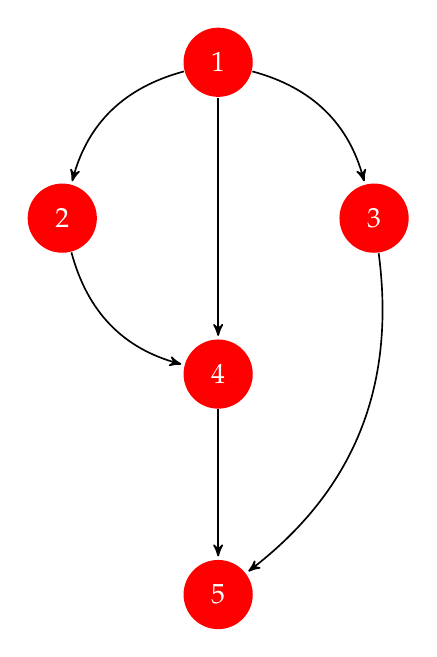
\begin{tikzpicture}[->,>=stealth',shorten >=1pt,auto,node distance=2.8cm,
                    semithick]
  \tikzstyle{every state}=[fill=red,draw=none,text=white]

  \node[state] (A)                    {1};              
  \node[state]         (B) [below right of=A] {3};
  \node[state]         (C) [below left  of=A] {2};
  \node[state]         (D) [below left of=B] {4};
  \node[state]         (E) [below of=D]       {5};



        
  \path (A) edge [bend left]  node {} (B)
            edge [bend right]   node {} (C)
            edge               node{}       (D)
        (C) edge [bend right] node{} (D) 
        (D) edge node{} (E)
        (B) edge [bend left] node{} (E)   
        ;      
\end{tikzpicture}
 
Fig.1: Revision diagram of Example 1. In the following diagram the nodes are the revisions. Outgoing arrows represent forks and  joins are represented by incoming arrows, which are always two, one straight for the revision we are joining to and one bend for the joinee. In the diagram nodes correspond to revisions as follows: 1 - {\tt revision } 2 - {\tt rev1 } 3 - {\tt rev2 } 4 - {\tt join\_rev1 } 5 - {\tt join\_rev2}  

\subsection{Illegal revision diagrams}
Not all possible joins are legal as some of them might invalidate the assumptions about the flow of revisions. Consider these examples of illegal diagrams:

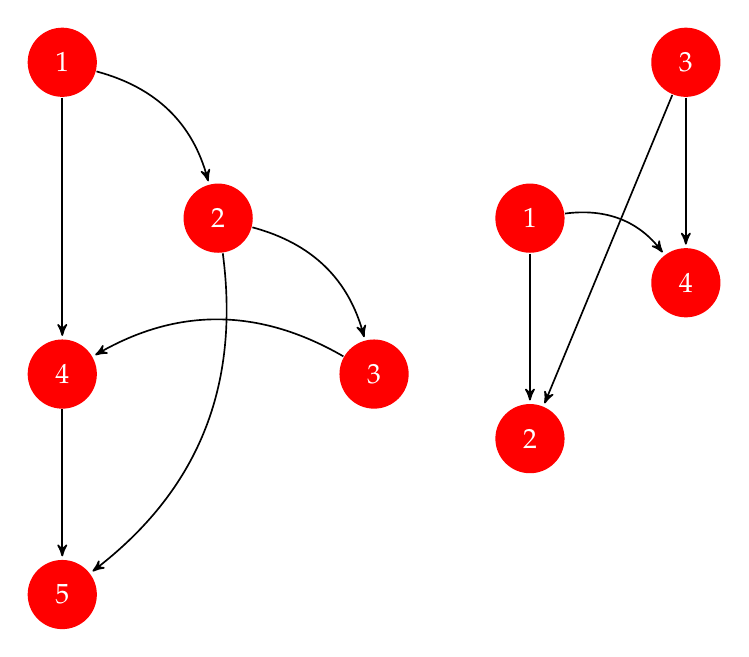
\begin{tikzpicture}[->,>=stealth',shorten >=1pt,auto,node distance=2.8cm,
                    semithick]
  \tikzstyle{every state}=[fill=red,draw=none,text=white]

  \node[state]         (A)                    {1};              
  \node[state]         (B) [below right of=A] {2};
  \node[state]         (C) [below right  of=B] {3};
  \node[state]         (D) [below left of=B] {4};
  \node[state]         (E) [below of=D]       {5};

  \node[state]         (F) [above right of=C]         {1};
  \node[state]        (G) [below of=F]         {2};
  \node[state]         (H) [above right of=F]         {3};
  \node[state]         (I) [below of=H]        {4};
        
  \path (A) edge [bend left]  node {} (B)
            edge               node{}       (D)
        (C) edge [bend right] node{} (D) 
        (D) edge node{} (E)
        (B) edge [bend left] node{} (C)
            edge [bend left] node{} (E)
            
        (F) edge node{} (G)
            edge [bend left] node{} (I)
        (H) edge node{} (I)
            edge  node{} (G)           
        ;      
\end{tikzpicture}
\\Fig.2: Illegal revision diagrams.
\vspace{10pt}

In Fig.2 we can see two illegal revision diagrams. In the first one, we join revision 3 to revision 1 before we have joined revision 2 which is the parent revision of 3. This means that the result in revision 5 might not be what we would expect as we are interleaving the joins and we might merge the work done in 2 effectively twice.

In the second example, we are interleaving two separate flows of revisions and there is no way to ensure that they isolate a similar state.

\subsection{Concurrent revisions in the world of OCaml}
The OCaml implementation of Concurrent Revisions is presented in chapter 3. One of its advantages over the C\# implementation is that it is purely functional and the type checker catches some of the typical mistakes that can be made - trying to access an isolated of a wrong type or join revisions of different types. What it does not do however is check for all types of illegal revision diagrams, instead an exception is raised whenever a illegal join is performed. This is far from ideal and statically type-checking joins for compatibility could be implemented as a future extension.

The API that the implementation exposes to the user is intuitive and resembles the typical OCaml approach for APIs for external libraries. Here is a simple example of its usage:

%module IntRevision = Make(struct
%    type t = int
%    let merge head parent current = head + current - parent
%  end)

%let () =
%  let r = IntRevision.init () in
%  let res1 = IntRevision.create r 0 in
%  let revision = IntRevision.get_revision res1 
%5  and account = IntRevision.get_isolated res1 in
%     Deferred.both (IntRevision.fork revision 
%        (fun r -> return (IntRevision.write r account ((IntRevision.read r account) + 5)))
%                   (IntRevision.fork revision 
%                      (fun r -> return (IntRevision.write r account ((IntRevision.read r account) + 10)))
%     >>|(fun (rev1, rev2 ->
%        let join_rev1 = IntRevision.join revision rev1 in
%        let join_rev2 = Intrevision.join join_rev1 rev2 in
%          assert(IntRevision.read join_rev2 = 15)  
\newpage

{\scriptsize\noindent\begin{longtable}{r|l}
\mlcodeline{1}{\mlkeywordA{module}~IntRevision~\mlkeyword{=}~Make(\mlkeyword{struct}
}
\mlcodeline{2}{~~~~\mlkeyword{type}~t~\mlkeyword{=}~int
}
\mlcodeline{3}{~~~~\mlkeywordA{let}~merge~head~parent~current~\mlkeyword{=}~head~\mloperator{+}~current~\mloperator{-}~parent
}
\mlcodeline{4}{~~\mlkeyword{end})
}
\mlcodeline{5}{
}
\mlcodeline{6}{\mlkeywordA{let}~()~\mlkeyword{=}
}
\mlcodeline{7}{~~\mlkeywordA{let}~r~\mlkeyword{=}~\mlmodulename{IntRevision}\mbox{}\mloperator{.}init~()~\mlkeywordA{in}
}
\mlcodeline{8}{~~\mlkeywordA{let}~res1~\mlkeyword{=}~\mlmodulename{IntRevision}\mbox{}\mloperator{.}create~r~0~\mlkeywordA{in}
}
\mlcodeline{9}{~~\mlkeywordA{let}~revision~\mlkeyword{=}~\mlmodulename{IntRevision}\mbox{}\mloperator{.}get\_{}revision~res1~
}
\mlcodeline{10}{~~\mlkeywordA{and}~account~\mlkeyword{=}~\mlmodulename{IntRevision}\mbox{}\mloperator{.}get\_{}isolated~res1~\mlkeywordA{in}
}
\mlcodeline{11}{~~~~~\mlmodulename{Deferred}\mbox{}\mloperator{.}both~(\mlmodulename{IntRevision}\mbox{}\mloperator{.}fork~revision~
}
\mlcodeline{12}{~~~~~~~~~~~~~~~~~~~~~(\mlkeyword{fun}~r~\mlkeyword{->}~return~(\mlmodulename{IntRevision}\mbox{}\mloperator{.}write~r~account~((\mlmodulename{IntRevision}\mbox{}\mloperator{.}read~r~account)~\mloperator{+}~5)))
}
\mlcodeline{13}{~~~~~~~~~~~~~~~~~~~(\mlmodulename{IntRevision}\mbox{}\mloperator{.}fork~revision~
}
\mlcodeline{14}{~~~~~~~~~~~~~~~~~~~~~(\mlkeyword{fun}~r~\mlkeyword{->}~return~(\mlmodulename{IntRevision}\mbox{}\mloperator{.}write~r~account~((\mlmodulename{IntRevision}\mbox{}\mloperator{.}read~r~account)~\mloperator{+}~10)))
}
\mlcodeline{15}{~~~~~\mloperator{>\mbox{}>\mbox{}|}(\mlkeyword{fun}~(rev1\mloperator{\mbox{,}}~rev2~\mlkeyword{->}
}
\mlcodeline{16}{~~~~~~~~\mlkeywordA{let}~join\_{}rev1~\mlkeyword{=}~\mlmodulename{IntRevision}\mbox{}\mloperator{.}join~revision~rev1~\mlkeywordA{in}
}
\mlcodeline{17}{~~~~~~~~\mlkeywordA{let}~join\_{}rev2~\mlkeyword{=}~\mlmodulename{Intrevision}\mbox{}\mloperator{.}join~join\_{}rev1~rev2~\mlkeywordA{in}
}
\mlcodeline{18}{~~~~~~~~~~\mlkeyword{assert}(\mlmodulename{IntRevision}\mbox{}\mloperator{.}read~join\_{}rev2~account~\mlkeyword{=}~15)}
\end{longtable}
}


Example 2.\\

In Example 2 we can see the actual implementation of the pseudo code in Example 1. From line 1 to 4 the user creates the {\tt IntRevision} module using a simple anonymous module specifying the type of the isolated data and the merge function. Then on line 7 he initializes an empty revision and one 8 and 9 he adds a new isolated to the initial revision to create a new one. He them forks the two asynchronous account credits (line 11 to 14) and later joins them. 

This API is not as straight forward as the one in the C\# implementations for couple of reasons. Firstly since it is purely functional, revisions are immutable which requires to create a new revision at each join. Secondly, we need to explicitly create new isolated variables. What is more, it does not allow having isolated from different types in a revision, a trivial workaround for which is to use tuples.  




\cleardoublepage



\chapter{Preparation}
\section{The author in the world of Concurrency}
As part of my degree I have gained broad knowledge of the problems that arise from Concurrency and the typical approaches for solving them. The Concurrent and Distributed Systems course gave me most insight into why and how Concurrent revisions can be used for parallel programming. After reading the original paper, the concept naturally fit in and expanded the mental model I have created about the issues and solutions in the world of Concurrency.  

\section{Familiarizing with the OCaml programming language}
Prior to starting the project, I had almost no experience with the OCaml programming language. For that reason I dedicated the first part of my project to making myself familiar with it. I used the Real World OCaml book [3] to guide me through the concepts and patterns for the language. I was able to quickly transfer and expand my skills in ML into OCaml without much difficulty.

\section{The Core and Async libraries}
I made extensive use of the Core and Async libraries for OCaml. The latter was used in the core of the implementation and the use cases. The Revision module conforms to the pattern of deferred computations in the Async library. This naturally happened in the development process, mainly because the library enforces them. Another reason for this is that the revision and isolated data types are completely isolated, making it trivial to implement them as deferred data types and the forks and the joins as deferred computations.  



\cleardoublepage
\chapter{Implementation}

\section{Nuts and Bolts}

Usage of the library is straight forward and effortless. The user first has to satisfy a module signature called {\tt Isolatable}:

{\scriptsize\noindent\begin{longtable}{r|l}
\mlcodeline{1}{\mlkeywordA{module}~\mlkeyword{type}~Isolatable~\mlkeyword{=}~\mlkeyword{sig}
}
\mlcodeline{2}{~~\mlcomments{(**~Type~{to}~be~isolated~**)}
}
\mlcodeline{3}{~~\mlkeyword{type}~t
}
\mlcodeline{4}{~~\mlcomments{(**~Merge~{function}{\mbox{\COLON}}~merge~{[}head{]}~{[}parent{]}~{[}current{]}~**)}
}
\mlcodeline{5}{~~\mlkeyword{val}~merge\mloperator{\mbox{\COLON}}~t~\mlkeyword{->}~t~\mlkeyword{->}~t~\mlkeyword{->}~t
}
\mlcodeline{6}{\mlkeyword{end}
}
\mlcodeline{7}{
}
\mlcodeline{8}{\mlkeywordA{module}~Make(X\mloperator{\mbox{\COLON}}Isolatable)~\mloperator{\mbox{\COLON}}~
}
\mlcodeline{9}{~~~~~~~~~~~~(Revision~\mlkeyword{with}~\mlkeyword{type}~value~\mlkeyword{=}~\mlmodulename{X}\mbox{}\mloperator{.}t~\mlkeywordA{and}~\mlkeyword{type}~isolated~\mlkeyword{=}~(int~\mloperator{*}~\mlmodulename{X}\mbox{}\mloperator{.}t)~\mlmodulename{Deferred}\mbox{}\mloperator{.}t)}
\end{longtable}
}

Then from this module, using the {\tt Make} functor, he create a {\tt Revision} module that satisfies the following signature:

{\scriptsize\noindent\begin{longtable}{r|l}
\mlcodeline{1}{\mlkeywordA{module}~\mlkeyword{type}~Revision~\mlkeyword{=}~\mlkeyword{sig}
}
\mlcodeline{2}{~~\mlkeyword{type}~i
}
\mlcodeline{3}{~~\mlkeyword{type}~result
}
\mlcodeline{4}{~~\mlkeyword{type}~t
}
\mlcodeline{5}{~~\mlkeyword{type}~isolated
}
\mlcodeline{6}{~~\mlkeyword{type}~value
}
\mlcodeline{7}{
}
\mlcodeline{8}{~~\mlkeyword{val}~init\mloperator{\mbox{\COLON}}~unit~\mlkeyword{->}~t
}
\mlcodeline{9}{~~\mlcomments{(**~Adds~a~{new}~isolated~{with}~{[}value{]}~{and}~returns~a~{new}~result~**)}
}
\mlcodeline{10}{~~\mlkeyword{val}~create\mloperator{\mbox{\COLON}}~~t~\mlkeyword{->}~value~\mlkeyword{->}~result
}
\mlcodeline{11}{~~
}
\mlcodeline{12}{~~\mlcomments{(**~For~breaking~the~result~into~revision~{and}~isolated~**)}
}
\mlcodeline{13}{~~\mlkeyword{val}~get\_{}revision\mloperator{\mbox{\COLON}}~result~\mlkeyword{->}~t
}
\mlcodeline{14}{~~\mlkeyword{val}~get\_{}isolated\mloperator{\mbox{\COLON}}~result~\mlkeyword{->}~isolated
}
\mlcodeline{15}{~~
}
\mlcodeline{16}{~~\mlcomments{(**~Scheduling~primitives~**)}
}
\mlcodeline{17}{~~\mlkeyword{val}~fork\mloperator{\mbox{\COLON}}~t~\mlkeyword{->}~(t~\mlkeyword{->}~t~\mlmodulename{Deferred}\mbox{}\mloperator{.}t)~\mlkeyword{->}~t~\mlmodulename{Deferred}\mbox{}\mloperator{.}t
}
\mlcodeline{18}{~~\mlkeyword{val}~join\mloperator{\mbox{\COLON}}~t~\mlkeyword{->}~t~\mlkeyword{->}~t
}
\mlcodeline{19}{~~
}
\mlcodeline{20}{~~\mlcomments{(**~Isolated~access~**)}
}
\mlcodeline{21}{~~\mlkeyword{val}~write\mloperator{\mbox{\COLON}}~t~\mlkeyword{->}~isolated~\mlkeyword{->}~value~\mlkeyword{->}~t
}
\mlcodeline{22}{~~\mlkeyword{val}~read\mloperator{\mbox{\COLON}}~t~\mlkeyword{->}~isolated~\mlkeyword{->}~value~option~\mlmodulename{Deferred}\mbox{}\mloperator{.}t
}
\mlcodeline{23}{
}
\mlcodeline{24}{\mlkeyword{end}}
\end{longtable}
}
 
Creation of revisions is done by the {\tt init} and {\tt create} functions. The former initializes an empty revision and the latter takes a revision and an initial value of the isolated type and returns a {\tt result}, which contains a tuple of {\tt Revision.t} and {\tt isolated}. This tuple can then be broken up by the usage of {\tt get\_revision} and {\tt get\_isolated}. This seems a bit awkward to use, but it is enforced by the Async library. Both {\tt Revision.t} and {\tt isolated} are deferred types, however since create takes a deferred type as first argument, it has to return a deferred type as well, meaning it cannot return a tuple of deferreds.

The scheduling primitives are the trivial {\tt fork} and {\tt join} operations common for asynchronous tasks. Note that they are both purely functional and do not mutate any of the input state and return a fresh revision each time. The right type of revision for these is type checked. For the illegal revision diagrams when the merge cannot reconcile a valid state, because there is not enough information in the revisions, an exception is raised. There are still some cases when the programmer can implement by error illegal schedules and run them successfully. Ideally these errors should be caught by the type checked or by a more elaborate dynamic runtime check. These are left as a future extension and for now such errors are considered programmer fault. 

Accessing the isolated variables is allowed by the {\tt write} and {\tt read} functions.
The former is also purely function and returns a new revision with the updated value. In the case when the isolated is not in this revision an exception will be raised [remove the option from read].

The internal structure of the revisions is implemented by the following data type:

{\scriptsize\noindent\begin{longtable}{r|l}
\mlcodeline{1}{\mlkeyword{type}~t~\mlkeyword{=}~\mloperator{\{}~parent~\mloperator{\mbox{\COLON}}~((int\mloperator{\mbox{,}}~\mlmodulename{Isolated}\mbox{}\mloperator{.}t\mloperator{\mbox{,}}~\mlmodulename{Int}\mbox{}\mloperator{.}comparator\_{}witness)~\mlmodulename{Map}\mbox{}\mloperator{.}t)\mloperator{\mbox{\SC}}
}
\mlcodeline{2}{~~~~~~~~~~~self~\mloperator{\mbox{\COLON}}~((int\mloperator{\mbox{,}}~\mlmodulename{Isolated}\mbox{}\mloperator{.}t\mloperator{\mbox{,}}~\mlmodulename{Int}\mbox{}\mloperator{.}comparator\_{}witness)~\mlmodulename{Map}\mbox{}\mloperator{.}t)\mloperator{\mbox{\SC}}
}
\mlcodeline{3}{~~~~~~~~~~~written~\mloperator{\mbox{\COLON}}~\mlmodulename{WrittenSet}\mbox{}\mloperator{.}t\mloperator{\mbox{\SC}}
}
\mlcodeline{4}{~~~~~~~~~~~id~\mloperator{\mbox{\COLON}}~int~
}
\mlcodeline{5}{~~~~~~~~~\mloperator{\}}~\mlmodulename{Deferred}\mbox{}\mloperator{.}t}
\end{longtable}
}

It is a deferred record type which contains two maps that map isolated variables to their to their value in the parent or the current revision respectfully. Their is also a written set that keeps track of which isolated variables have been updated in order to improve the performance at join time. The {\tt Isolated.t} is itself implemented simply as an integer value that is used as a key into the maps. The {\tt id} field in the revision type keeps track of the id of the last created isolated in that revision chain.    

\section{Design decisions and complexity}

The key aims of the design were to produce a solution that is purely functional, as well as efficient.

The main design choice for the implementation was how to implement the revisions internally. The obvious choice for the mapping of isolated variables to values was either using hash tables or maps. The former would have given us constant time for all the update and add operations. However, they are imperative which would have broken the functional model of their operation. We could have hidden under the curtains the fact we are using a mutable data structure by lazy replication, which however would have increased the space complexity by the order of number of revisions times the number of isolated variables. Given that the functional nature that we were aiming for, which required creating a new revision after each operation, this was highly undesirable. Instead the choice of using maps was made. Since only insertion and update operations were performed on the maps, all operations on maps we use are of logarithmic time. What is more, since maps in OCaml are purely functional, they reuse a lot of their internal structure and there is no duplication of data. This results in space complexity of order of the sum of the number of revisions and the number of isolated writes. 

All operations on revisions were implemented as deferred computations in the framework of the Async library. This makes the Concurrent revisions easy to integrate in any application using the idioms of the Async library, which is one of the mainstream parallel frameworks for OCaml.

Reads, writes and {\tt create} take logarithmic time, as they effectively are operations on a map. Forking takes constant time and joins take time O(klgn) where n is the number of isolated variables and k is the number of written values inside the fork.     

 
\section{Use cases}
\subsection{Chat server}

 
 
 why it is usefull to do it that way (trivial problem, but doing it in this framework is interesting and could show much)
structure \& implementation (briefly)
experimental data - a lot of chat rooms, merging chatrooms, conflicts; some plots could be good
sequential version (hopefully) – compare both
   
\subsection{Other one?}

\section{Remaining issues}






\cleardoublepage
\chapter{Evaluation}

\section{Fitness of the concept for the use cases}
Was it easy to implement them in that way? Did it make me thing in a different way (was it better)? What was exceptionally good about it?

\section{Negative aspects}
Any syntactic of conceptual awkwardness encountered along the way

\section{Performance evaluation}
\subsection{Experimental data}
Plots, analyzes, etc.

\subsection{Performance analyzes}
Time, space, what seem to be a bottle neck, were the design choices right? 




\cleardoublepage
\chapter{Conclusion}

It works! (or not)




\cleardoublepage

%%%%%%%%%%%%%%%%%%%%%%%%%%%%%%%%%%%%%%%%%%%%%%%%%%%%%%%%%%%%%%%%%%%%%
% the bibliography

\addcontentsline{toc}{chapter}{Bibliography}
\bibliography{refs}
\cleardoublepage
\chapter{Bibliography}
\begin{description}
\item{[1]} \emph{Concurrent Programming with Revisions and Isolation Types}, Sebastian Burckhardt, Alexandro Baldassion, and Daan Leijen. OOPSLA'10
\item{[2]} \emph{Source repository:} https://github.com/dpp23/ocaml\_revisions
\item{[3]} \emph{Real World OCaml} Jason Hickey, Anil Madhavapeddy, and Yaron Minsky; O'Reilly 2013
\item{[4]} \emph{Concurrency Control and Recovery in Database Systems. Addison-Wesley, 1987} P.A.Bernstein, V.Hadzilacos, and N.Goodman.

\end{description}

%%%%%%%%%%%%%%%%%%%%%%%%%%%%%%%%%%%%%%%%%%%%%%%%%%%%%%%%%%%%%%%%%%%%%
% the appendices
\appendix


\chapter{Project Proposal}

%\input{propbody}

\end{document}
